
% ---
% Inserir folha de aprovação
% ---

% Isto é um exemplo de Folha de aprovação, elemento obrigatório da NBR
% 14724/2011 (seção 4.2.1.3). Você pode utilizar este modelo até a aprovação
% do trabalho. Após isso, substitua todo o conteúdo deste arquivo por uma
% imagem da página assinada pela banca com o comando abaixo:
%
%\begin{folhadeaprovacao}
%	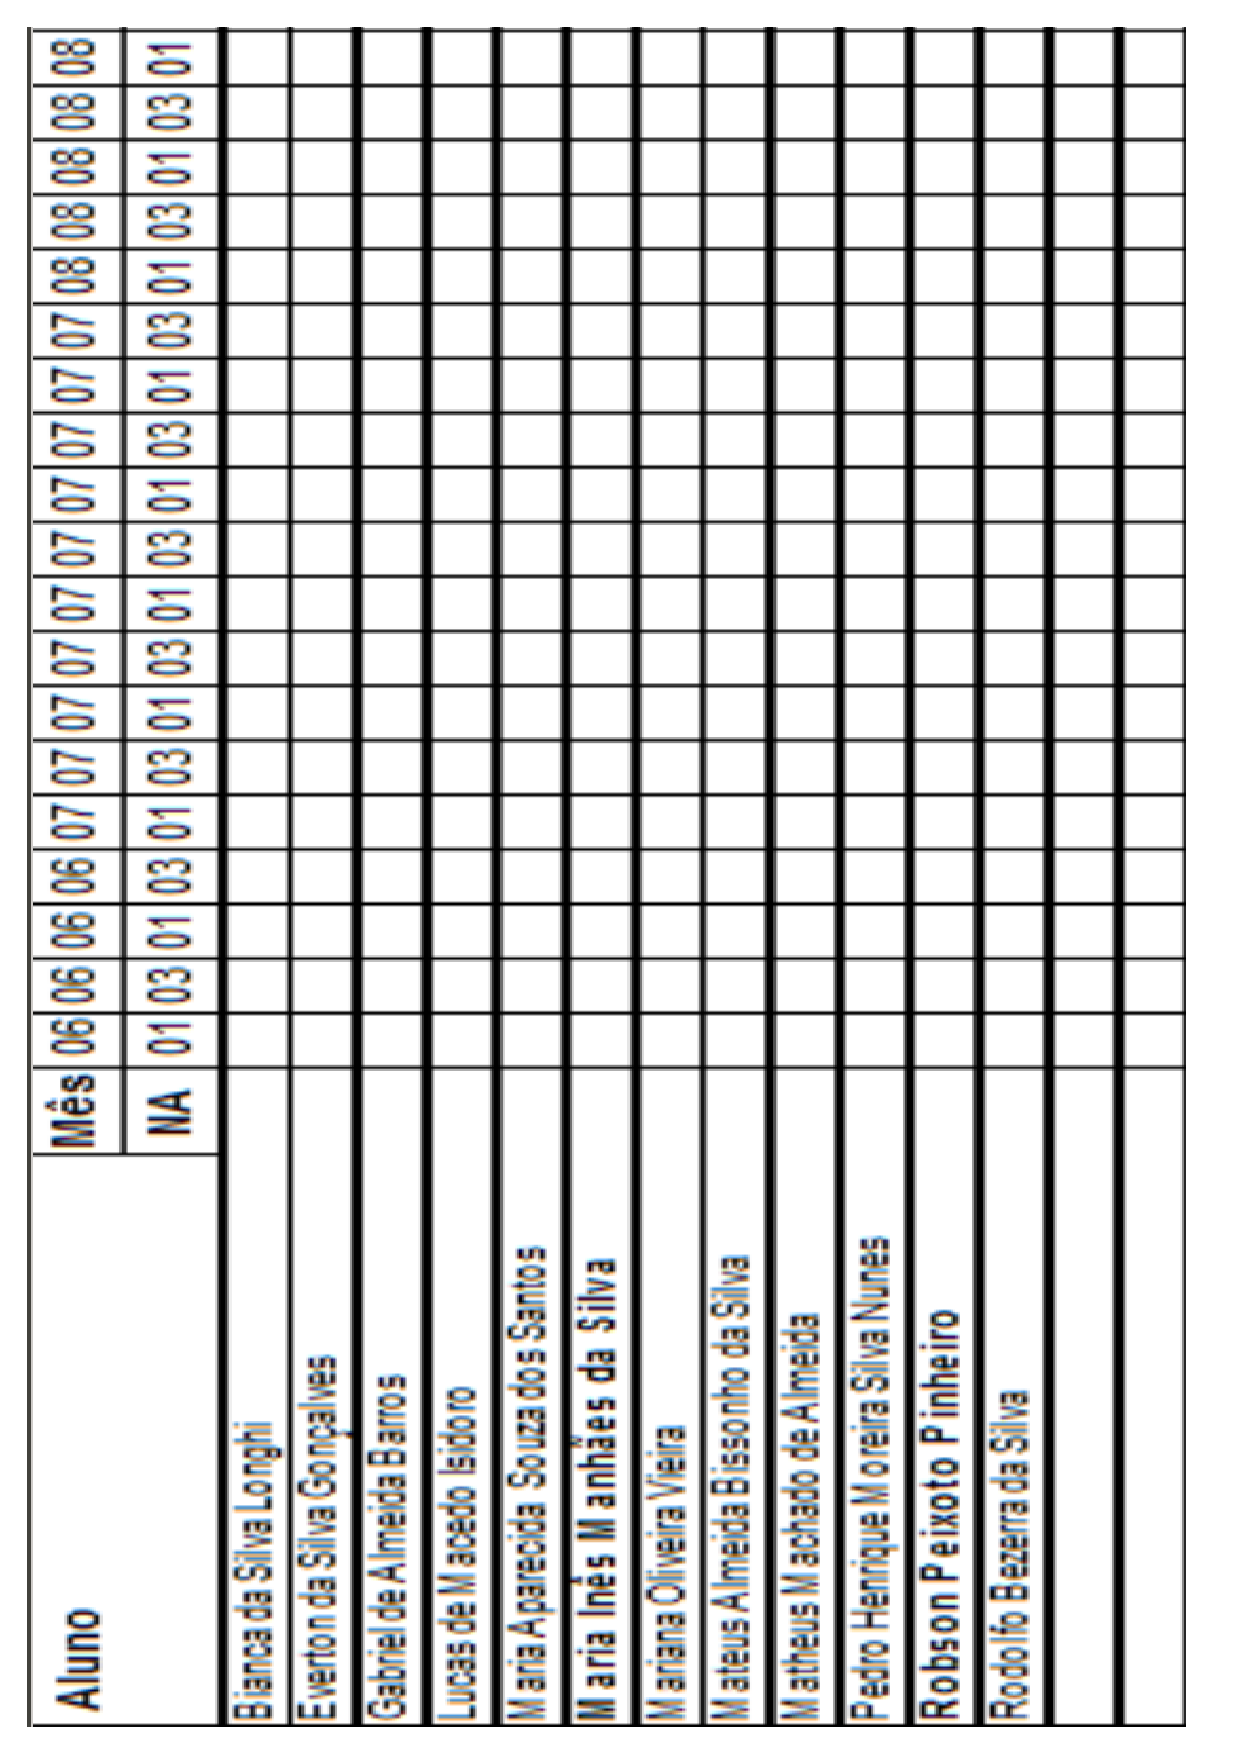
\includepdf{pre/FolhaAprovacaoAssinada}
%\end{folhadeaprovacao}

%
\begin{folhadeaprovacao}

\setlength{\ABNTEXsignwidth}{14cm}

    \begin{center}
    {\ABNTEXchapterfont\large\imprimirautor}

    \vspace*{\fill}\vspace*{\fill}
    {\ABNTEXchapterfont\bfseries\Large\imprimirtitulo}
    \vspace*{\fill}
    
    \hspace{.45\textwidth}
    \begin{minipage}{.5\textwidth}
        \imprimirpreambulo
    \end{minipage}%
    \vspace*{\fill}
   
   \end{center}
 
 
   \begin{center}
    \imprimirlocal, \imprimirdia ~de \imprimirmes ~de \imprimirano.
   \end{center}
   
   % Instituto Federal Fluminense (IFF)
   \assinatura{\textbf{Prof. M.Sc. Nome do Primeiro Professor} \\ Instituto Federal Fluminense (IFF)}
   \assinatura{\textbf{Prof. D.Sc. Nome do Segundo Professor} \\ Universidade Estadual do Norte Fluminense - Darcy Ribeiro (UENF)}
   \assinatura{\textbf{\imprimirorientador} \\ Instituto Federal Fluminense (IFF)}
   \assinatura{\textbf{\imprimircoorientador} \\ Instituto Federal Fluminense (IFF)}

   \begin{center}
    \vspace*{0.5cm}
    {\ABNTEXchapterfont\large\imprimirlocal}
    \par
    {\ABNTEXchapterfont\large\imprimirdata}
    \vspace*{1cm}
  \end{center}
  
\end{folhadeaprovacao}
% ---
